\documentclass[10pt]{article}
\usepackage{fullpage,enumitem,amsmath,amssymb,graphicx,listings,tikz,bbm,xcolor}
\setlength{\parindent}{0pt}

\begin{document}

\begin{center}
{\Large \textbf{Homework 7: Car Tracking}}

\begin{tabular}{rl}
\\
Course: & CS 221 Spring 2019 \\
Name: & Bryan Yaggi
\end{tabular}
\end{center}

\section*{\normalsize Problem 1: Bayesian Network Basics}

First, let us look at a simplified version of the car tracking problem. For this problem only, let $C_t \in \{0,1\}$ be the actual location of the car we wish to observe at time step $t \in \{1,2,3\}$. Let $D_t \in \{0,1\}$ be a sensor reading for the location of that car measured at time $t$. Here's what the Bayesian network (it's an HMM, in fact) looks like:

\begin{center}
  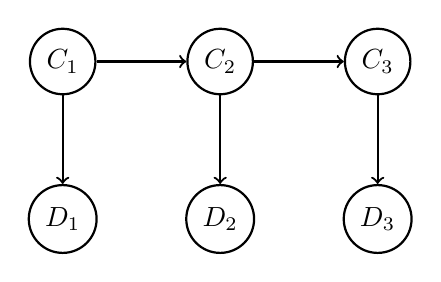
\begin{tikzpicture}
		\begin{scope}[every node/.style={circle,thick,draw}]
    		\node (C1) at (0,2) {$C_1$};
    		\node (C2) at (2,2) {$C_2$};
    		\node (C3) at (4,2) {$C_3$};
    		\node (D1) at (0,0) {$D_1$};
    		\node (D2) at (2,0) {$D_2$};
    		\node (D3) at (4,0) {$D_3$};
		\end{scope}
		\begin{scope}[every edge/.style={draw=black,thick}]
			\path [->] (C1) edge node {} (D1);	    		
    		\path [->] (C2) edge node {} (D2);
    		\path [->] (C3) edge node {} (D3);
    		\path [->] (C1) edge node {} (C2);
    		\path [->] (C2) edge node {} (C3);
		\end{scope}
	\end{tikzpicture}
\end{center}

The distribution over the initial car distribution is uniform; that is, for each value $c_1 \in \{0,1\}$:
$$p(c_1) = 0.5$$

The following local conditional distribution governs the movement of the car (with probability $\epsilon$, the car moves). For each $t \in \{2,3\}$:
$$p(c_t \mid c_{t-1}) = \begin{cases}
	\epsilon &\text{if} \ c_t \neq c_{t-1}\\
	1 - \epsilon &\text{if} \ c_t = c_{t-1}
\end{cases}$$

The following local conditional distribution governs the noise in the sensor reading (with probability $\eta$, the sensor reports the wrong position). For each $t \in \{1,2,3\}$:
$$p(d_t \mid c_t) = \begin{cases}
	\eta &\text{if} \ d_t \neq c_t\\
	1 - \eta &\text{if} \ d_t = c_t
\end{cases}$$

Below, you will be asked to find the posterior distribution for the car's position at the second time step ($C_2$) given different sensor readings.
\smallskip

Important: For the following computations, try to follow the general strategy described in lecture (marginalize non-ancestral variables, condition, and perform variable elimination). Try to delay normalization until the very end. You'll get more insight than trying to chug through lots of equations.

\begin{enumerate}[label=(\alph*)]

  \item Suppose we have a sensor reading for the second timestep, $D_2 = 0$. Compute the posterior distribution $\mathbb{P}(C_2 = 1 \mid D_2 = 0)$. We encourage you to draw out the (factor) graph.
  
  \begin{center}
	  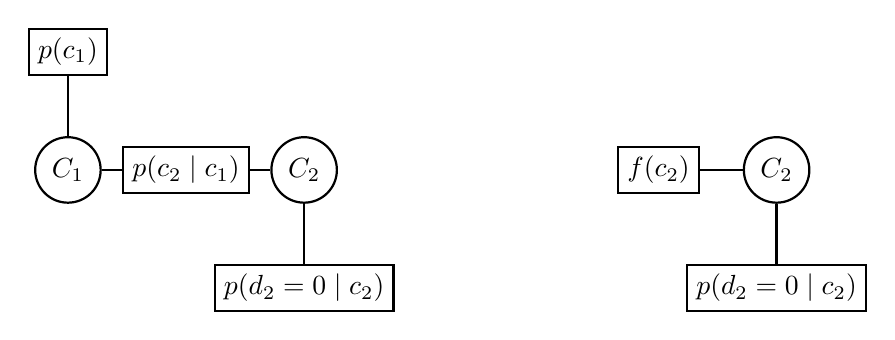
\begin{tikzpicture}
			\begin{scope}[every node/.style={circle,thick,draw}]
	    		\node (C11) at (0,3) {$C_1$};
	    		\node (C21) at (3,3) {$C_2$};
	    		\node (C22) at (9,3) {$C_2$};
			\end{scope}
			\begin{scope}[every node/.style={rectangle,thick,draw}]
	    		\node (f0) at (0,4.5) {$p(c_1)$};
	    		\node (f1) at (1.5,3) {$p(c_2 \mid c_1)$};
	    		\node (f21) at (3,1.5) {$p(d_2 = 0 \mid c_2)$};
	    		\node (f3) at (7.5,3) {$f(c_2)$};
	    		\node (f22) at (9,1.5) {$p(d_2 = 0 \mid c_2)$};
			\end{scope}
			\begin{scope}[every edge/.style={draw=black,thick}]
				\path [-] (f0) edge node {} (C11);	    		
	    		\path [-] (C11) edge node {} (f1);
	    		\path [-] (f1) edge node {} (C21);
	    		\path [-] (C21) edge node {} (f21);
	    		\path [-] (f3) edge node {} (C22);
	    		\path [-] (C22) edge node {} (f22);
			\end{scope}
		\end{tikzpicture}
	\end{center}

	\begin{align*}
	f(c_2) &= \sum_{c_1} p(c_1) p(c_2 \mid c_1) = \begin{cases}
	.5 (1 - \epsilon) + .5\epsilon = .5 &\text{if} \ c_2 = 0\\
	.5 \epsilon + .5 (1 - \epsilon) = .5 &\text{if} \ c_2 = 1
	\end{cases}\\
	\mathbb{P}(C_2 = c_2 \mid D_2 = 0) &\propto f(c_2) p(d_2 = 0 \mid c_2) = \begin{cases}
	.5(1 - \eta) &\text{if} \ c_2 = 0\\
	.5\eta &\text{if} \ c_2 = 1
	\end{cases}\\
	\mathbb{P}(C_2 = 1 \mid D_2 = 0) &= \eta
	\end{align*}
  
  \item Suppose a time step has elapsed and we got another sensor reading, $D_3 = 1$, but we are still interested in $C_2$. Compute the posterior distribution $\mathbb{P}(C_2 = 1 \mid D_2 = 0, D_3 = 1)$. The resulting expression might be moderately complex. We encourage you to draw out the (factor) graph.
  
  \begin{center}
	  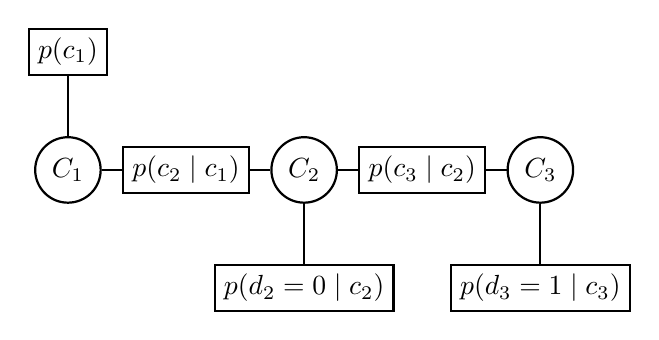
\begin{tikzpicture}
			\begin{scope}[every node/.style={circle,thick,draw}]
	    		\node (C1) at (0,3) {$C_1$};
	    		\node (C2) at (3,3) {$C_2$};
	    		\node (C3) at (6,3) {$C_3$};
			\end{scope}
			\begin{scope}[every node/.style={rectangle,thick,draw}]
	    		\node (f0) at (0,4.5) {$p(c_1)$};
	    		\node (f1) at (1.5,3) {$p(c_2 \mid c_1)$};
	    		\node (f2) at (3,1.5) {$p(d_2 = 0 \mid c_2)$};
	    		\node (f3) at (4.5,3) {$p(c_3 \mid c_2)$};
	    		\node (f4) at (6,1.5) {$p(d_3 = 1 \mid c_3)$};
			\end{scope}
			\begin{scope}[every edge/.style={draw=black,thick}]
				\path [-] (f0) edge node {} (C1);	    		
	    		\path [-] (C1) edge node {} (f1);
	    		\path [-] (f1) edge node {} (C2);
	    		\path [-] (C2) edge node {} (f2);
	    		\path [-] (C2) edge node {} (f3);
	    		\path [-] (f3) edge node {} (C3);
	    		\path [-] (C3) edge node {} (f4);
			\end{scope}
		\end{tikzpicture}
	\end{center}
	
	\begin{center}
	  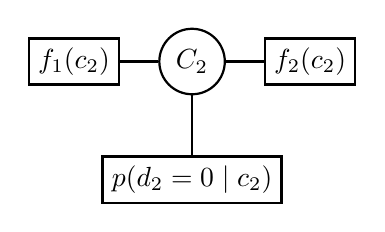
\begin{tikzpicture}
			\begin{scope}[every node/.style={circle,thick,draw}]
	    		\node (C2) at (3,3) {$C_2$};
			\end{scope}
			\begin{scope}[every node/.style={rectangle,thick,draw}]
	    		\node (f5) at (1.5,3) {$f_1(c_2)$};
	    		\node (f2) at (3,1.5) {$p(d_2 = 0 \mid c_2)$};
	    		\node (f6) at (4.5,3) {$f_2(c_2)$};
			\end{scope}
			\begin{scope}[every edge/.style={draw=black,thick}]
	    		\path [-] (f5) edge node {} (C2);
	    		\path [-] (C2) edge node {} (f2);
	    		\path [-] (C2) edge node {} (f6);
			\end{scope}
		\end{tikzpicture}
	\end{center}
	
	\begin{align*}
	f_1(c_2) &= \sum_{c_1} p(c_1) p(c_2 \mid c_1) = \begin{cases}
	.5 (1 - \epsilon) + .5\epsilon = .5 &\text{if} \ c_2 = 0\\
	.5 \epsilon + .5 (1 - \epsilon) = .5 &\text{if} \ c_2 = 1
	\end{cases}\\
	f_2(c_2) &= \sum_{c_3} p(c_3 \mid c_2) p(d_3 = 1 \mid c_3) = \begin{cases}
	(1 - \epsilon)\eta + \epsilon(1 - \eta) &\text{if} \ c_2 = 0\\
	\epsilon\eta + (1 - \epsilon)(1 - \eta) &\text{if} \ c_2 = 1
	\end{cases}\\
	\mathbb{P}(C_2 = c_2 \mid D_2 = 0, D_3 = 1) &\propto f_1(c_2) p(d_2 = 0 \mid c_2) f_2(c_2) = \begin{cases}
	.5(1 - \eta)((1 - \epsilon)\eta + \epsilon(1 - \eta)) &\text{if} \ c_2 = 0\\
	.5\eta(\epsilon\eta + (1 - \epsilon)(1 - \eta)) &\text{if} \ c_2 = 1
	\end{cases}\\
	\mathbb{P}(C_2 = 1 \mid D_2 = 0, D_3 = 1) &= \frac{\epsilon\eta^2 + (1 - \epsilon)(1 - \eta)\eta}{\epsilon\eta^2 + 2(1 - \epsilon)(1 - \eta)\eta + \epsilon(1 - \eta)^2}
	\end{align*}
		
	\item Suppose $\epsilon = 0.1$ and $\eta = 0.2$.
	\begin{enumerate}[label=(\roman*)]
		\item Compute and compare the probabilities $\mathbb{P}(C_2 = 1 \mid D_2 = 0)$ and $\mathbb{P}(C_2 = 1 \mid D_2 = 0, D_3 = 1)$. Give numbers, round your answer to 4 significant digits.
		
		\begin{align*}
		\mathbb{P}(C_2 = 1 \mid D_2 = 0) &= .2\\
		\mathbb{P}(C_2 = 1 \mid D_2 = 0, D_3 = 1) &= .4157
		\end{align*}
		
		\item How did adding the second sensor reading $D_3 = 1$ change the result? Explain your intuition for why this change makes sense in terms of the car positions and associated sensor observations.
		
		It increased the probability that $C_2 = 1$. Additional data is given that supports $C_2 = 1$. Since the probability that the position changes between timesteps is small, having the sensor reading $D_3 = 1$ makes it more likely that $C_2 = 1$. 
		
		\item What would you have to set $\epsilon$ while keeping $\eta = 0.2$ so that $\mathbb{P}(C_2 = 1 \mid D_2 = 0) = \mathbb{P}(C_2 = 1 \mid D_2 = 0, D_3 = 1)$? Explain your intuition in terms of the car positions with respect to the observations.
		
		$$\epsilon = .5$$
		
		This is effectively making it equally likely for $C_3$ to be 0 or 1 which makes knowing $D_3 = 1$ irrelevant.
		
	\end{enumerate}

\end{enumerate}
\iffalse
\section*{\normalsize Problem 1: CSP Solving}

\begin{enumerate}[label=(\alph*)]

  \item coding
  
  \item coding
  
  \item coding

\end{enumerate}

\section*{\normalsize Problem 2: Handling N-ary Factors}

So far, our CSP solver only handles unary and binary factors, but for course scheduling (and really any non-trivial application), we would like to define factors that involve more than two variables. It would be nice if we could have a general way of reducing n-ary constraint to unary and binary constraints. In this problem, we will do exactly that for two types of n-ary constraints.
\smallskip

Suppose we have boolean variables $X_1, X_2, X_3$, where $X_i$ represents whether the $i$-th course is taken. Suppose we want to enforce the constraint that $Y = X_1 \vee X_2 \vee X_3$, that is, $Y$ is a boolean representing whether at least one course has been taken. For reference, in \texttt{util.py}, the function \texttt{get\_or\_variable()} does such a reduction. It takes in a list of variables and a target value, and returns a boolean variable with domain $[True, False]$ whose value is constrained to the condition of having at least one of the variables assigned to the target value. For example, we would call \texttt{get\_or\_variable()} with arguments $(X_1, X_2, X_3, True)$, which would return a new (auxiliary) variable $X_4$, and then add another constraint $[X_4 = True]$.
\smallskip

The second type of n-ary factors are constraints on the sum over $n$ variables. You are going to implement reduction of this type but let's first look at a simpler problem to get started:

\begin{enumerate}[label=(\alph*)]

  \item Suppose we have a CSP with three variables $X_1, X_2, X_3$ with the same domain $\{ 0, 1, 2 \}$ and a ternary constraint $[X_1 + X_2 + X_3 \leq K]$. How can we reduce this CSP to one with only unary and/or binary constraints? Explain what auxiliary variables we need to introduce, what their domains are, what unary/binary factors you'll add, and why your scheme works. Add a graph if you think that'll better explain your scheme.
  
  Define a new variables $A_i, B_i$.
	\begin{align*}
		A_i &= A_{i-1} + X_i, A_0 = 0\\
		B_i &= (A_{i-1}, A_i)\\
  		Domain(B_i) &= \{ (x,y) : 0 \leq x \leq 6, 0 \leq y \leq 6, x \in \mathbb{Z}, y \in \mathbb{Z} \}
	\end{align*}	  
  
  
  Factors:
  \begin{itemize}
  		\item $\mathbbm{1}[B_1[0] = 0]$
  		\item $\mathbbm{1}[B_3[1] \leq K]$
  		\item $\mathbbm{1}[B_i[0] = B_{i-1}[1]]$
  		\item $\mathbbm{1}[B_i[1] = B_{i-1} + X_i]$
  \end{itemize}
  
  \begin{center}
	  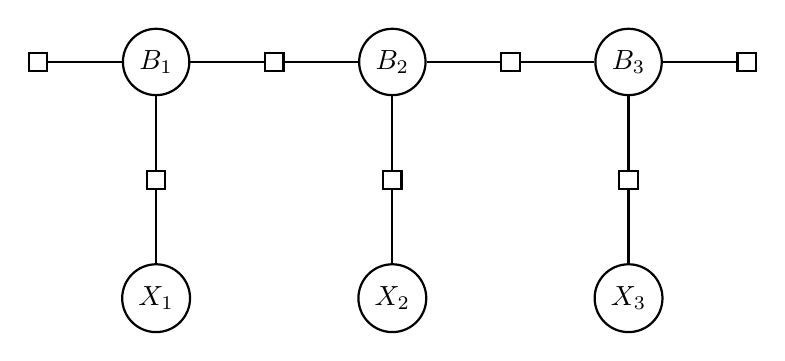
\begin{tikzpicture}
			\begin{scope}[every node/.style={circle,thick,draw}]
	    		\node (B1) at (3,0) {$B_1$};
	    		\node (B2) at (6,0) {$B_2$};
	    		\node (B3) at (9,0) {$B_3$};
	    		\node (X1) at (3,-3) {$X_1$};
	    		\node (X2) at (6,-3) {$X_2$};
	    		\node (X3) at (9,-3) {$X_3$};
			\end{scope}
			\begin{scope}[every node/.style={rectangle,thick,draw}]
				\node (t0) at (1.5,0)	 {};  		
	    		\node (t1) at (4.5,0) {};
	    		\node (t2) at (7.5,0) {};
	    		\node (t3) at (10.5,0) {};
	    		\node (t4) at (3,-1.5) {};
	    		\node (t5) at (6,-1.5) {};
	    		\node (t6) at (9,-1.5) {};
			\end{scope}
	
			\begin{scope}[every edge/.style={draw=black,thick}]
				\path [-] (t0) edge node {} (B1);	    		
	    		\path [-] (B1) edge node {} (t1);
	    		\path [-] (t1) edge node {} (B2);
	    		\path [-] (B2) edge node {} (t2);
	    		\path [-] (t2) edge node {} (B3);
	    		\path [-] (B3) edge node {} (t3);
	    		\path [-] (B1) edge node {} (t4);	    		
	    		\path [-] (t4) edge node {} (X1);
	    		\path [-] (B2) edge node {} (t5);
	    		\path [-] (t5) edge node {} (X2);
	    		\path [-] (B3) edge node {} (t6);
	    		\path [-] (t6) edge node {} (X3);
			\end{scope}
		\end{tikzpicture}
	\end{center}
  
  \item coding

\end{enumerate}

\section*{\normalsize Problem 3: Course Scheduling}

In this problem, we will apply your weighted CSP solver to the problem of course scheduling. We have scraped a subset of courses that are offered from Stanford's Bulletin. For each course in this dataset, we have information on which quarters it is offered, the prerequisites (which may not be fully accurate due to ambiguity in the listing), and the range of units allowed. You can take a look at all the courses in \texttt{courses.json}. Please refer to \texttt{util.Course} and \texttt{util.CourseBulletin} for more information. 

\begin{enumerate}[label=(\alph*)]

  \item coding
  
  \item coding
  
  \item Now try to use the course scheduler for the winter and spring (and next year if applicable). Create your own \texttt{profile.txt} and then run the course scheduler:

	\texttt{python run\_p3.py profile.txt}

	You might want to turn on the appropriate heuristic flags to speed up the computation. Does it produce a reasonable course schedule? Please include your \texttt{profile.txt} and the best schedule in your writeup; we're curious how it worked out for you!

	\texttt{profile.txt}\\
	\texttt{-----------}\\
	\texttt{minUnits 3}\\
	\texttt{maxUnits 5}\\
	\texttt{taken STATS116}\\
	\texttt{taken CS106A}\\
	\texttt{taken CS106B}\\
	\texttt{taken CS103}\\
	\texttt{taken CS107}\\
	\texttt{taken CS109}\\
	\texttt{taken CS110}\\
	\texttt{taken CS221}\\
	\texttt{request CS161 weight 2}\\
	\texttt{request CS231N weight 2}\\
	\texttt{request CS229}\\
	\texttt{request CS230}\\
	\texttt{request CS234}\\
	\texttt{-----------}

	Resulting best schedule:\\
		\begin{tabular}{l l l}
			Quarter & Units & Course\\
			\hline
	  		Sum2019 & 5 & CS161\\
	  		Aut2019 & 4 & CS229\\
	  		Win2020 & 3 & CS234\\
	  		Spr2020 & 4 & CS231N\\
	  	\end{tabular}
	  	
	  	Note: I added CS230, CS231N, and CS234 to \texttt{courses.json}.

\end{enumerate}

\section*{\normalsize Problem 4: Weighted CSPs with Notable Patterns (Extra Credit)}

Want more challenges about CSP? Here we go. :D
\smallskip

Suppose we have a weighted CSP with variables $X_1, \dots, X_n$ with domains $Domain_i = {1, \dots, K}$. We have a set of basic factors which depend only on adjacent pairs of variables in the same way: there is some function $g$ such that $f_i(x) = g(x_i, x_{i+1})$ for $i = 1, \dots, n−1$. In addition, we have a small set of notable patterns $P$, where each $p \in P$ is a sequence of elements from the domain.
\smallskip

Let $n_p$ be the number of times that $p$ occurs in an assignment $x = (x_1, \dots, x_n)$ as a consecutive sequence. Define the weight of an assignment $x$ to be $\prod_{i=1}^{n−1} f_i(x) \prod_{p \in P} \gamma^{n_p}$. Intuitively, we multiply the weight by $\gamma$ every time a notable pattern appears.
\smallskip

For example, suppose $n = 4$, $\gamma = 7$, $g(a,b)= 5[a = b] + 1[a \neq b]$ and $P = \{[1,3,3],[1,2,3]\}$. Then the assignment $x = [1,3,3,2]$ has weight $(1 \cdot 5 \cdot 1) \cdot (71 \cdot 70) = 35$. 

\begin{enumerate}[label=(\alph*)]

  \item If we were to include the notable patterns as factors into the CSP, what would be the worst case treewidth? (You can assume each $p$ has a maximum length of $n$.)
  
  \begin{center}
	  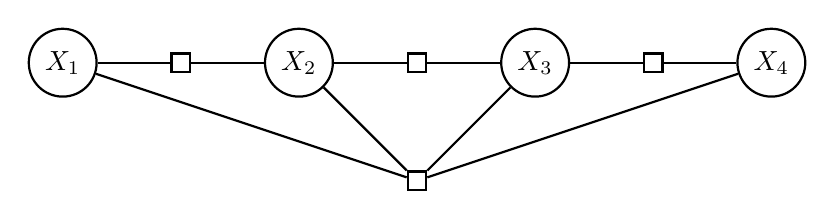
\begin{tikzpicture}
			\begin{scope}[every node/.style={circle,thick,draw}]
	    		\node (X1) at (1.5,0) {$X_1$};
	    		\node (X2) at (4.5,0) {$X_2$};
	    		\node (X3) at (7.5,0) {$X_3$};
	    		\node (X4) at (10.5,0) {$X_4$};
			\end{scope}
			\begin{scope}[every node/.style={rectangle,thick,draw}]
				\node (t0) at (3,0)	 {};  		
	    		\node (t1) at (6,0) {};
	    		\node (t2) at (9,0) {};
	    		\node (t3) at (6,-1.5) {};
			\end{scope}
	
			\begin{scope}[every edge/.style={draw=black,thick}]
				\path [-] (X1) edge node {} (t0);	    		
	    		\path [-] (t0) edge node {} (X2);
	    		\path [-] (X2) edge node {} (t1);
	    		\path [-] (t1) edge node {} (X3);
	    		\path [-] (X3) edge node {} (t2);
	    		\path [-] (t2) edge node {} (X4);
	    		\path [-] (X1) edge node {} (t3);
	    		\path [-] (X2) edge node {} (t3);
	    		\path [-] (X3) edge node {} (t3);
	    		\path [-] (X4) edge node {} (t3);
			\end{scope}
		\end{tikzpicture}
	\end{center}
	
	Worst-case tree width is $n - 1$.
  
  \item The treewidth doesn't really tell us the true complexity of the problem. Devise an efficient algorithm to compute the maximum weight assignment. You need to describe your algorithm in enough detail but don't need to implement it. Analyze your algorithm's time and space complexities. You'll get points only if your algorithm is much better than the naive solution.
		
\end{enumerate}
\fi
\end{document}
